\section{Arquitectura del sistema}

El presente hito documenta las decisiones arquitectónicas que sustentan el desarrollo 
del sistema, tanto en el backend como en el frontend. Comprender estas decisiones es 
fundamental para interpretar correctamente el código implementado en los hitos 
siguientes.

% -------------------------------------------------------
\subsection{Arquitectura del backend}

\subsubsection*{DTOs, Repositorios y Controladores}

El backend se organiza en torno a tres entidades que dividen responsabilidades de 
forma clara y evitan que una sola capa concentre demasiada lógica.

Un \textbf{DTO} (Data Transfer Object) es un objeto que define la estructura de los 
datos que viajan entre el backend y el cliente. Su función es actuar como contrato 
explícito: determina qué campos se exponen en una respuesta, qué campos son 
obligatorios al crear un recurso y cuáles son opcionales al actualizarlo. En este 
proyecto los DTOs se implementan como clases \texttt{SQLAlchemyDTO} que se vinculan 
directamente al modelo ORM, con una configuración \texttt{SQLAlchemyDTOConfig} que 
indica qué campos excluir o marcar como opcionales. Esta aproximación evita escribir 
esquemas de validación duplicados y garantiza coherencia entre el modelo de datos y 
el contrato de la API.

Un \textbf{repositorio} encapsula el acceso a los datos de una tabla. En este proyecto 
se utiliza \texttt{SQLAlchemySyncRepository} de Advanced Alchemy como base, que 
provee operaciones genéricas ya implementadas: \texttt{list}, \texttt{get\_one}, 
\texttt{add}, \texttt{get\_and\_update} y \texttt{delete}. Cuando la lógica de un 
módulo requiere operaciones que van más allá de estas primitivas, se crean 
\textbf{repositorios personalizados} extendiendo la clase base. La necesidad de 
personalización surge cuando una operación involucra múltiples tablas en una misma 
transacción, requiere cargar relaciones mediante \texttt{selectinload} para evitar 
consultas N+1, o debe aplicar lógica de negocio antes de persistir, como el hashing 
de contraseñas o la actualización coordinada de estados entre tablas vinculadas.

Un \textbf{controlador} define los endpoints HTTP del recurso. Hereda de 
\texttt{Controller} de Litestar y declara los métodos decorados con 
\texttt{@get}, \texttt{@post}, \texttt{@patch} y \texttt{@delete}, cada uno 
correspondiente a una operación CRUD. El controlador no contiene lógica de acceso a 
datos: su responsabilidad es recibir la petición, inyectar las dependencias necesarias 
(repositorio, usuario autenticado) y delegar la operación al repositorio. La 
transformación de los datos de entrada y salida queda a cargo de los DTOs, que 
Litestar aplica automáticamente al serializar y deserializar las respuestas.

La delegación entre estas tres entidades sigue siempre el mismo flujo: el 
\textbf{controlador} recibe la petición y valida el acceso; el \textbf{DTO} 
transforma y valida los datos; y el \textbf{repositorio} ejecuta la operación sobre 
la base de datos. Esta separación hace que cada capa sea independientemente legible, 
testeable y reemplazable.

\subsubsection*{Estructura de directorios y concepto de servicio}

Los módulos del backend se ubican en \texttt{app/services/labdic\_inventory/}. Cada 
subdirectorio representa un módulo funcional del sistema y contiene, de forma 
consistente, los archivos \texttt{dtos.py}, \texttt{repositories.py} y 
\texttt{controllers.py}. El término \textit{servicio} se utiliza aquí en un sentido 
arquitectónico amplio: Se refiere al conjunto de componentes (DTO, repositorio y 
controlador) que implementan la funcionalidad de un módulo. Esta convención de 
nomenclatura refleja que cada directorio entrega una capacidad completa del sistema, 
desde el acceso a datos hasta la exposición de la API.

\subsubsection*{Router del backend}

En \texttt{app/services/labdic\_inventory/router.py} se define \texttt{labdic\_inventory\_router}, 
una instancia de \texttt{Router} de Litestar con el prefijo de ruta 
\texttt{/labdic\_inventory}. Este router agrupa todos los controladores del sistema 
bajo un prefijo común, de modo que los endpoints de cada módulo quedan organizados 
bajo rutas como \texttt{/labdic\_inventory/users}, \texttt{/labdic\_inventory/products}, 
etcétera. En \texttt{app/main.py}, este router se registra como único manejador de 
rutas de la aplicación Litestar, junto con los plugins de SQLAlchemy y seguridad. 
El router existe porque centraliza la configuración de rutas y permite aplicar 
prefijos, middlewares o políticas de seguridad a nivel de grupo sin tener que 
repetirlos en cada controlador individual.

% -------------------------------------------------------
\subsection{Arquitectura del frontend}

\subsubsection*{Router, control de acceso y \texttt{RouterView}}

El router del frontend se configura en \texttt{src/router/index.ts} mediante 
\texttt{createRouter} de Vue Router. Cada ruta asocia una URL a un componente de 
vista y puede llevar metadatos como \texttt{requiresAuth: true} o 
\texttt{requiresAdmin: true}. El guard global definido en \texttt{beforeEach} 
consulta las stores antes de cada cambio de ruta: si el usuario no está autenticado, 
redirige al login preservando la URL de destino; si no tiene privilegios de 
administrador, redirige al home. La directiva \texttt{<RouterView />} actúa como 
punto de montaje dinámico en los layouts: el router sustituye este elemento con el 
componente de vista que corresponde a la ruta activa, sin recargar el resto del 
layout.

\subsubsection*{Stores, Pinia y \texttt{localStorage}}

Pinia es la librería oficial de gestión de estado global para Vue 3. En este proyecto 
se utiliza para mantener dos stores persistentes entre recargas de página: 
\texttt{useAuthStore} y \texttt{useUserStore}.

\texttt{useAuthStore} almacena el token JWT en \texttt{localStorage} y expone la 
propiedad computada \texttt{isAuthenticated}. Al iniciar la aplicación, el token se 
recupera automáticamente del almacenamiento local, lo que permite que el usuario 
permanezca autenticado sin necesidad de iniciar sesión nuevamente tras una recarga. 
Cuando el token expira o el usuario cierra sesión, \texttt{clearToken} lo elimina 
tanto del estado reactivo como del \texttt{localStorage}.

\texttt{useUserStore} almacena el objeto completo del usuario autenticado, incluyendo 
sus roles. También persiste en \texttt{localStorage} para que propiedades como 
\texttt{isAdmin} estén disponibles inmediatamente al recargar, sin necesidad de hacer 
una petición adicional al backend. Expone propiedades computadas como \texttt{isAdmin}, 
\texttt{isUser} y métodos auxiliares como \texttt{hasRole} y \texttt{hasAnyRole}, 
que son consumidos tanto por el router como por los componentes de la interfaz para 
mostrar u ocultar elementos según el rol del usuario.

El uso de \texttt{localStorage} en lugar de cookies de sesión es una decisión 
deliberada: simplifica la implementación en un entorno de desarrollo local y es 
coherente con el flujo de autenticación basado en Bearer tokens de la API.

\subsubsection*{Carpeta \texttt{types/} y contrato con la API}

La carpeta \texttt{src/types/} contiene las interfaces TypeScript que definen la 
estructura de los datos que el frontend espera recibir o enviar a la API. Estas 
interfaces son el equivalente frontend de los DTOs del backend: establecen un 
contrato de tipos que el compilador puede verificar en tiempo de desarrollo, 
reduciendo errores de integración. Por ejemplo, \texttt{device.types.ts} define la 
interfaz \texttt{Device} con todos los campos que expone \texttt{DeviceReadDTO}, y 
\texttt{DevicePayload} con los campos requeridos para crear o actualizar un 
dispositivo.

Un aspecto importante es la conversión de nomenclatura: el backend retorna JSON con 
claves en \texttt{snake\_case} (convención de Python), mientras que el frontend 
trabaja en \texttt{camelCase} (convención de TypeScript). La función \texttt{apiFetch} 
en \texttt{src/services/api.ts} aplica esta conversión automáticamente en ambas 
direcciones usando la librería \texttt{change-case/keys}: convierte las claves del 
cuerpo enviado a \texttt{snake\_case} antes de hacer la petición, y convierte las 
claves de la respuesta recibida a \texttt{camelCase} antes de retornarla. Esto 
permite que las interfaces en \texttt{types/} usen \texttt{camelCase} de forma 
consistente sin que los componentes deban preocuparse por la convención del backend.

\subsubsection*{Carpeta \texttt{services/} y función \texttt{apiFetch}}

La carpeta \texttt{src/services/} centraliza las funciones que realizan peticiones 
HTTP a la API. Cada archivo corresponde a un módulo del sistema 
(\texttt{user.service.ts}, \texttt{device.service.ts}, \texttt{loan.service.ts}, 
etcétera) y exporta funciones con nombres descriptivos como \texttt{getDevices}, 
\texttt{createLoan} o \texttt{deleteProduct}. Todas estas funciones delegan en 
\texttt{apiFetch}, la función central definida en \texttt{src/services/api.ts}.

\texttt{apiFetch} cumple varias responsabilidades de forma transversal: adjunta 
automáticamente el header \texttt{Authorization: Bearer \{token\}} si el usuario 
está autenticado, serializa el cuerpo de la petición a JSON con conversión de claves 
a \texttt{snake\_case}, deserializa la respuesta con conversión a \texttt{camelCase}, 
maneja el código de respuesta \texttt{204 No Content} para operaciones de eliminación, 
y ante un error \texttt{401} limpia las stores y redirige al login indicando que la 
sesión expiró. Esta centralización evita repetir la lógica de autenticación y manejo 
de errores en cada llamada individual, y garantiza un comportamiento consistente en 
toda la aplicación.

La razón de tener una carpeta \texttt{services/} separada de las vistas es de 
separación de responsabilidades: los componentes Vue no deben conocer los detalles 
del protocolo HTTP ni la estructura exacta de las URLs. Al delegar en los servicios, 
los componentes solo necesitan llamar a \texttt{getDevices()} o 
\texttt{createLoan(payload)} y recibir datos ya tipados, sin acoplarse a la 
infraestructura de comunicación.

% -------------------------------------------------------
\subsection{Flujo de consumo de la API}\label{sec:flujo_api}

El flujo completo desde la base de datos hasta la interfaz de usuario puede 
describirse en cuatro capas que se articulan de forma secuencial.

\textbf{Capa de datos.} PostgreSQL actúa como motor relacional. SQLAlchemy mapea 
las tablas a clases Python mediante el ORM declarativo, y \texttt{database.py} 
conecta PostgreSQL con Litestar a través de \texttt{SQLAlchemySyncConfig}, que 
recibe la cadena de conexión \texttt{postgresql+psycopg2:///labdic\_inventory} 
desde la configuración del proyecto y registra el plugin de SQLAlchemy en la 
aplicación. Alembic se integra con el mismo modelo de SQLAlchemy para gestionar 
las migraciones versionadas del esquema, manteniendo la base de datos sincronizada 
con el código a lo largo del desarrollo.

\textbf{Capa de API.} Litestar expone los datos a través de la API REST. 
\texttt{SQLAlchemySyncRepository} provee el acceso a datos desde los controladores, 
y \texttt{SQLAlchemyDTO} transforma los modelos ORM en respuestas JSON con los 
campos adecuados según el contexto. La seguridad se gestiona en \texttt{security.py} 
mediante \texttt{OAuth2PasswordBearerAuth}, que intercepta cada petición, valida el 
token JWT y resuelve el usuario autenticado antes de que el controlador ejecute la 
operación solicitada. Todas las rutas quedan agrupadas bajo el prefijo 
\texttt{/labdic\_inventory} a través del router del backend.

\textbf{Puente frontend-backend.} La carpeta \texttt{types/} define las interfaces 
TypeScript que representan los DTOs del backend en el lado del cliente, estableciendo 
el contrato de tipos. La carpeta \texttt{services/} implementa las funciones que 
consumen la API usando \texttt{apiFetch}, que se encarga de adjuntar el token de 
autenticación, convertir las claves entre \texttt{snake\_case} y \texttt{camelCase}, 
y manejar los errores de forma centralizada. La URL base del backend 
(\texttt{http://localhost:8000}) se configura en \texttt{api.ts}, y el backend 
permite las peticiones del frontend mediante la configuración de CORS en 
\texttt{main.py}.

\textbf{Capa de presentación.} En el frontend, Pinia gestiona el estado global 
persistido en \texttt{localStorage}: el token JWT en \texttt{useAuthStore} y los 
datos del usuario autenticado en \texttt{useUserStore}. Vue Router controla la 
navegación y el acceso a las rutas usando la información de las stores. Los módulos 
del frontend, organizados por funcionalidad, consumen los servicios para obtener 
datos y los presentan a través de componentes de PrimeVue y TailwindCSS, garantizando 
una interfaz coherente y adaptable.

El diagrama de la figura~\ref{fig:flujo_api} sintetiza este flujo de forma visual.

\begin{figure}[H]
	\centering
	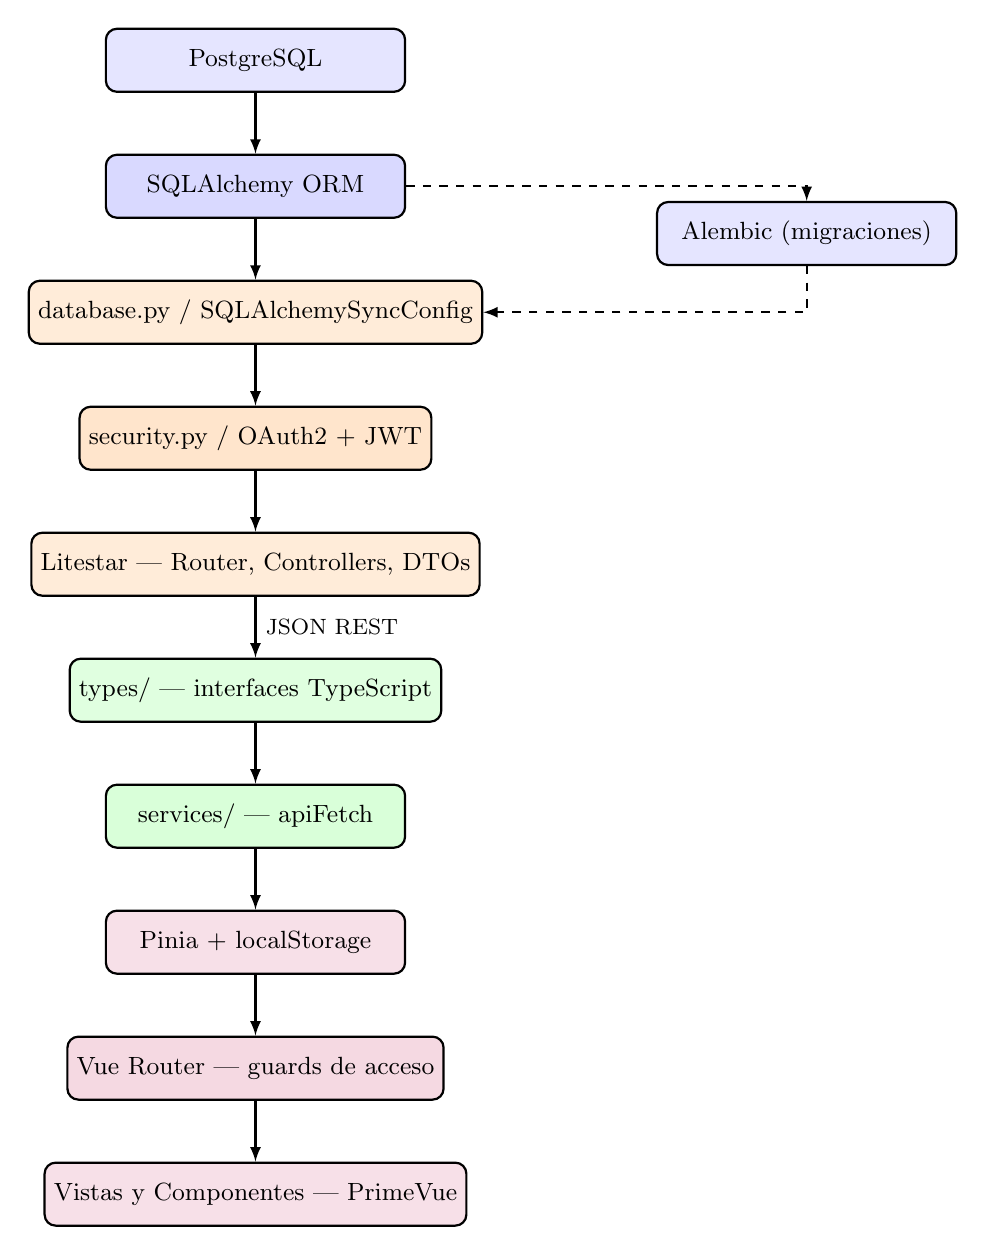
\begin{tikzpicture}[
		every node/.style={font=\small},
		box/.style={
			draw, thick, rounded corners=4pt,
			minimum width=3.8cm, minimum height=0.8cm,
			align=center,
		},
		arrow/.style={->, thick, >=latex},
		]
		
		\node[box, fill=blue!10]   (postgres)   at (0,  0)    {PostgreSQL};
		\node[box, fill=blue!15]   (sqlalchemy) at (0, -1.6)  {SQLAlchemy ORM};
		\node[box, fill=blue!10]   (alembic)    at (7.0, -2.2) {Alembic (migraciones)};
		\node[box, fill=orange!15] (database)   at (0, -3.2)  {database.py / SQLAlchemySyncConfig};
		\node[box, fill=orange!20] (security)   at (0, -4.8)  {security.py / OAuth2 + JWT};
		\node[box, fill=orange!15] (litestar)   at (0, -6.4)  {Litestar — Router, Controllers, DTOs};
		\node[box, fill=green!12]  (types)      at (0, -8.0)  {types/ — interfaces TypeScript};
		\node[box, fill=green!15]  (services)   at (0, -9.6)  {services/ — apiFetch};
		\node[box, fill=purple!12] (stores)     at (0,-11.2)  {Pinia + localStorage};
		\node[box, fill=purple!15] (router)     at (0,-12.8)  {Vue Router — guards de acceso};
		\node[box, fill=purple!12] (views)      at (0,-14.4)  {Vistas y Componentes — PrimeVue};
		
		\draw[arrow] (postgres)   -- (sqlalchemy);
		\draw[arrow] (sqlalchemy) -- (database);
		\draw[arrow] (database)   -- (security);
		\draw[arrow] (security)   -- (litestar);
		\draw[arrow] (litestar)   -- node[right, font=\footnotesize]{JSON REST} (types);
		\draw[arrow] (types)      -- (services);
		\draw[arrow] (services)   -- (stores);
		\draw[arrow] (stores)     -- (router);
		\draw[arrow] (router)     -- (views);
		
		\draw[->, thick, >=latex, dashed]
		(sqlalchemy.east) -| (alembic.north);
		\draw[->, thick, >=latex, dashed]
		(alembic.south) |- (database.east);
		
	\end{tikzpicture}
	\caption{Flujo de consumo de la API del sistema LabDIC.}
	\label{fig:flujo_api}
\end{figure}